\chapter{Methods and Implementations} \label{ch:Methods}
\section{Overview}
In this chapter we'll discuss the design decisions we've made in detail.  We
have 3 distinct phases.  The first phase, preprocessing, is converting the data files into a unified dataset in memory and configuring for the following phases.  The second phase is the hybrid approach where we optimize external classifiers,followed by the purist approach where we use our genetic algorithm (GA) to develop classification rules.  Each of these approaches generate confusion matrices which we analyze.\\
The general flow of the algorithm can be seen in \ref{fig:ProgramFlow}. 
\begin{figure}
	\centering
	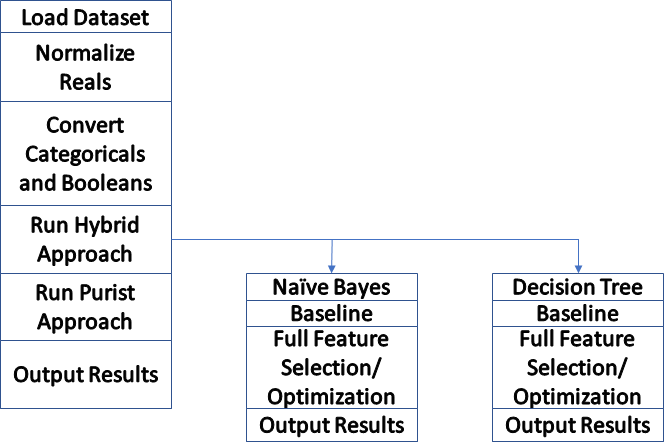
\includegraphics[width=0.7\linewidth]{figures/png/ProgramFlow}
	\caption[Overall Program Flow]{Birds-eye view of the flow of the program.
		Hybrid approaches are not run in parallel, because at time of coding MATLAB
		doesn't support multi-threading via a COM server.}
	\label{fig:ProgramFlow}
\end{figure}
Loading and normalization gets all algorithms on the same page, ensuring an
apples-to-apples comparison.  First we have the hybrid approaches.  Within a
hybrid approach, we first see what optimizing without including features yields; this is referred to in the code and in the program as the baseline approach.  It
has all the same constraints as the parent approach.  After the baseline, we
optimize a second time, this time including feature selection, by which we mean
that we characterize a dataset with n variables as either included (1) or
excluded (0) in a bitstring, and encode the same variables to the classifier as
in the baseline method.  We have selected two distinct classifiers: a multiclass
na\"ive Bayes algorithm and a simple single decision tree.  Each of these are
run twice per dataset, once with feature selection disabled (the baseline) and
once with it enabled.  We will discuss those methods in more detail in their
respective sections.\\The purist approach is much more straightforward.  There
is only one mode which it runs in, there's no explicit feature selection.  That
is, there is feature selection, but all features are available to the algorithm
at any time, though some may not be included. This portion of the algorithm
is threaded.  
\section{Preprocessing}
We do some preprocessing of the data.  First and foremost, there is a text file
that is read which describes the dataset and points to where it is on the
filesystem.  Below is an example which tells the program where it can find X and
Y and how to parse them.\pagebreak
\begin{lstlisting}[language=config, caption={Cardio Config File}, label={fig:config}]
#Dataset Name
CardioData
#Class Names File
../../../Data/Cardio/classNames.txt
#TrainingSet X Path
../../../Data/Cardio/trainingXY.csv
#TrainingSet Y Path
../../../Data/Cardio/trainingXY.csv
#TestingSet  X Path
../../../Data/Cardio/testingXY.csv
#TestingSet  Y Path
../../../Data/Cardio/testingXY.csv
#X ignore list, comma separated and starting with w if it's a whitelist
(otherwise, blacklist)
b, 29, 30
#Y ignore list, as above
w, 29
#Categorical Variables, white/blacklist, comma separated
w, 
#Boolean Variables, as above
w, 
\end{lstlisting}

For instance, in this case X(the data) and Y(the labels) are in the same file,
but represented as different columns.  They could easily be stored as two files.
After those files are explained, the next uncommented line describes the
columns to ignore or include, specified with b for blacklist or w for whitelist
respectively.  In this example, columns 29 and 30 are ignored for X, but only 29
is included for Y.  This is because for this dataset, there are two sets of
labels and thus two separate description files to use the file differently. 
Using the same notation, we can declare categorical and boolean variables for X.
Y is assumed to be categorical.\\
After we read how to parse the file, we read the files themselves.  At this
point we also convert booleans and categorical variables to doubles so that they
can fit in the same matrix.  First, however, we want to normalize the Reals. 
First we gather max, min and mean from each column in the dataset.  Then we use
a function to squeeze the values down between .1 (b) and .9 (t) for reasons that
will be seen later in the section on the purist approach.  
$$x_i^{\prime} = b+(t-b)\frac{(x^i-x_i^{min})}{x_i^{max}-x_i^{min}}$$ Next,
categorical variables are given the treatment motivated and described fully in
\cite{zhang_visual_2015}, the conclusion being that every category label is
replaced with a real number which maximizes Pearson's Correlation Coefficient. 
That is,
\begin{align*}
	X &= {X_\mathbb{R} \cup X_{cat} \cup X_{bool}}\\
X_\mathbb{R} &= \{\textbf{x}_1, \textbf{x}_2, ... \textbf{x}_n\}\\
X_{cat} &= \{\textbf{x}_{n+1}, \textbf{x}_{n+2}, ... \textbf{x}_c\}\\%there are some number of categorical columns,
%each of which have a number of categoricals in them.
X_{bool} &= \{\textbf{x}_{c+1}, \textbf{x}_{c+2,} ... \textbf{x}_b\} \\
1&\leq i \leq c-n\\
L &= \{x_i|\textbf{x}_i\epsilon X_{cat}\}\\%Set of categoricals
C_\ell &= \{\textbf{x}, i|  \textbf{x}\epsilon X \wedge \textbf{x}_{n+i} = \ell\epsilon L \}\\%set of samples
%belonging to categoricals
\end{align*}
Where X is the dataset, $X_\mathbb{R}$ is the real portion of the dataset, and$
X_{cat}$ and $X_{bool}$ are the categorical and boolean portions.  The index $i$
iterates over the columns of $X_{cat}$, which lets us derive L, which is the set
of all categories in the dataset.  L in turn gives us a means of devising $C_\ell$,
that is, the subset of X which consists of all members of x which belong to the
category $\ell$. Now it is possible to look at $C_\ell$ and determine which values
will maximize $r^2$ for each label $\ell$, which we here call $R(\ell)$.
\begin{align}
	R(\ell) &= \frac{\sum_{\textbf{x}\epsilon C_\ell}\sum_{j=1}^{n}x_j}{|C_\ell|n}
\end{align} 
It can be seen as the mean of all the other values over $C_\ell$.  Calculating this
in practice is much more straightforward: simply step through X one sample at a
time, and maintain running sums and counts for each unique label, calculate the
means at the end and then extend $X_\mathbb{R}$ with the newly calculated
values.  In the case of multiple categorical columns, unless there is a perfect
correlation between two category labels each label will have its own value
(though this can't be proven to be unique, only generated from a unique set of
numbers).\\
Booleans are only given the treatment of being converted to values .25 for false
and .75 for true.  Again, the reasons we don't use 0 and 1.0 will be made clear
in the section on our purist approach.\\
Now that the data has been modified, some additional bookkeeping is
accomplished.  Conversions to numerics from string class labels and vice versa
are computed and stored, since mathematical approaches prefer integers while
human-readable outputs are in the terms given us by the dataset.  Also, global
values such as Elitism Percentage and Population Size are modified at this point
and are effectively constant for the rest of the program.  Variables that may be
configured by the user are: Max Generations, Record Interval, Population Size,
and Complexity bounds.  The Max Generations sets the stopping condition of the
algorithms, and defaults to 100.  The Record Interval determines how often to
save data to the disk. Data is collected every generation, but is only saved to
disk in where $G \mod(I) = 0$, and the default value of I is 25.  Complexity bounds are
discussed in more detail in the purist approach, and have no effect on the
hybrid approach.  Other modifications to semi-constants are made at this point
determining the length of chromosomes for both approaches based on the
characteristics of the datasets, particularly the number of features and number of classes.
\section{Hybrid Approach}
As mentioned previously, the hybrid approach consists of 2 methods which each
consist of two different ways of running them.  First we will discuss the
multi-class na\"ive Bayes (McNB) approach, followed by the decision tree (DTree)
approach.
\paragraph{McNB}
Na\"ive Bayes is one of the most basic of classifiers, but it is powerful and
versatile.  Without going into extreme detail, it generates probability
distributions for each class across every dimension in the feature set from the
training data, and picks the most likely class for a given sample point. 
Typically, the probability distributions are Gaussian, however any density
function can be used.   We use this because it should provide a fairly low bar
to compete against; support vector machines (SVMs) are much more complex, tend to
be extremely reliable and robust, and are close to something resembling the
industry standard, but don't perform well with multiple classes.  McNB is closer
to statistical modeling and is not what we consider machine learning, though no
bright line distinction exists.  It is a theoretically grounded but simple
statistical method well suited to being a first pass at the data or being used
in conjunction with other methods.  Being simple, it is also relatively fast-
only 2 passes through the data are necessary to build the parameters for the
PDFs, so building the model can be done in linear time.  Once built, checking a
given variable can be done in constant time.
\begin{equation}
P(A|B) = \frac{P(B|A)*P(A)}{P(B)}
\end{equation}
While that is the standard formulation of Bayes' theorem, in our case it is more useful to reframe it thus\footnote{Thanks to Dr. Hairong Qi for teaching this formulation.}:
\begin{equation}
P(\omega_j|\textbf{x}) = \frac{p(\textbf{x}|\omega_j)P(\omega_j)}{p(\textbf{x})}
\label{eq:bayes}
\end{equation}
Here, $P(\omega_j|x)$ is the likelihood of $x$ belonging to a particular class.  Upper
case $P$s are simple probabilities, lower case $p$s are more complex functions.
So $p(x|\omega_j)$ is the PDF, and $P(\omega_j)$ is the prior, which can be
thought of as \textit{a priori} how likely a particular class is to present.  To
build the PDF, if we're using a Gaussian, we need mean and standard deviation
for each class.  The Gaussian PDF is built using the training set, tested on the
testing set, and the results are scored in a confusion matrix.  This can be
determined from the dataset, in which case it uses the frequency in the Training
set to generate priors, or set manually.  In either case, this can be seen to
scale a particular PDF.  In fact, this is similar to what $p(\textbf{x})$ does except
that where $P(\omega_j)$ scales a class, $p(\textbf{x})$ scales all classes, and it
serves as a normalizing factor to constrain values between 0 and 1.  It could
be established using the law of total probability, or it could be some
arbitrarily high constant\footnote{It doesn't really make a difference, since the selected class will just be the one with the highest score given x. 	Furthermore, if it affects all classes equally nothing is served by making
complex calculations every time the classifier is called.  Simply calculate the highest value it could take initially and use that in subsequent calls.}.  Thus, the specifics of $p(\textbf{x})$ are largely irrelevant for our purposes.  Rather, we will focus on the parameters to the MATLAB classifier we invoke. \\Our implementation, which we'll refer to as the McNB optimizer\footnote{To avoid confusion, our optimizers are optimizing classifiers, they are not classifiers but optimizers.  Later, we present our classifier.} optimizes the fitcnb  \footnote{For much further
detail on Mathworks' implementation see
\url{http://www.mathworks.com/help/stats/fitcnb.html}.} function in MATLAB over the following parameters: distribution, kernel, score transform, and priors.  Further, it optimizes over the dataset by choosing which features are included.  It is entirely defined by its bitstring, the first several bits correspond one-to-one to the features in the dataset.  An optimizer with all 1s (or all 0s to avoid having no data) will include the entire dataset.  Otherwise, a 1 indicates that the column is included, a 0 removed.
  \\
The distribution uses 2 bits and can be any of the following values:\\
\begin{itemize}
	\item Kernel uses a smoothing function, described below.\item	Multinomial represents every class as a single multinomial distribution.
	\item	Multivariate multinomial characterizes each feature as an independent
	multinomial distribution based on the unique values found in the feature.
	\item	Normal distributions behave as described above.
\end{itemize}
Kernel type uses two bits, though these go unused unless the distribution is
kernel.  Then the variables are smoothed via various functions outlined below.
\begin{itemize}
	\item \textbf{Box} uses a uniform, box-like smoothing window.
	\item \textbf{Epanechnikov} is a very efficient, rounded kernel.  Minimizes
	Asymptotic Mean Integrated Square Error (AMISE)\citep{stefanie_scheid_introduction_2004} therefore optimal
	in that sense.
	\item \textbf{Gaussian} is a standard normal function but used in this case for
	smoothing.
	\item \textbf{Triangular} is another form of smoothing, with a peak of 1 at 0
	and zero at -1 and 1.
\end{itemize}
Regardless of which form of smoothing, the goal is the same:  to create a
distribution of a random variable which can then be modeled.  This is done using
something like a histogram, which is then smoothed into a continuous function
using the kernel chosen above.  This becomes $p(x|\omega_j)$ in the equation
\ref{eq:bayes}.\\
For priors, each class extends our optimizer's bit length by 3 bits.  Each class
then has a prior in the range  $1 + [0,8]= [1,9]$ which is later summed and turned into a
probability distribution summing to unity.  For instance, if a database has 2 classes, and an optimizer has assigned one a prior of 3 and the other a prior of 7, these are converted
into percentages of 30\% and 70\%, respectively.  These become the $P(\omega_j)$ in equation \ref{eq:bayes}.\\
Finally, the score transform takes up 3 bits and can be any of eight values. 
This is used internally in the MATLAB function.  It can take on any of the following
values:
\begin{itemize}
	\item DoubleLogit transforms the score to $\frac{1}{1+e^{-2x}}$
	\item Invlogit $\log(\frac{x}{1-x})$
	\item Logit $\frac{1}{1+e^{-x}}$
	\item None $x$
	\item Sign $\frac{x}{|x|}$, or 0 when x = 0.
	\item Symmetric $2x-1$
	\item Symmetricismax 1 if max of class, 0 otherwise
	\item Symmetriclogit $\frac{2}{1+e^{-x}}-1$
\end{itemize}
Once these are determined, the optimizer is evaluated.  This means that the training set is passed to the optimizer, it is trained, and then the testing set is passed to it, from which we get the fitness of the classifier.  Fitness is average accuracy.  That is, suppose we have a confusion matrix C\\
C= \begin{tabular}{|c|c|c|c|c|}
	\hline
	True:&$\omega_1$&$\omega_2$&$\omega_3$&\textbf{Total}\\
	\hline
	Predicted $\omega_1$&4&6&5&\textbf{15}\\
	\hline
	Predicted $\omega_2$&2&2&9&\textbf{13}\\
	\hline
	Predicted $\omega_3$&8&2&110&\textbf{120}\\
	\hline
	Total&\textbf{14}&\textbf{10}&\textbf{124}&\textbf{148}\\
	\hline
\end{tabular} 
\\The dataset in this case has 3 classes, $\omega_1$, $\omega_2$, and $\omega_3$, and has 148 total samples.  Of those, 14 are class $\omega_1$, 10 are class $\omega_2$, and 124 are class $\omega_3$.  Meanwhile, the classifier predicted that 15 of the samples were $\omega_1$, 13 were $\omega_2$, and 120 were $\omega_3$.  To determine accuracy, the equation is $\frac{\sum_{i=1}^{3}C_{ii}}{148}$.  This is a good metric for relatively evenly distributed classes.  However, in highly skewed cases as this one, this treats more rare classes as less important.  For instance, in this case, the accuracy is $\frac{116}{148} = 0.784$, which might seem like it is doing a decent job, and maybe it is, if the concern is finding Cs.  Average accuracy is slightly more complicated to calculate, but still straightforward enough.  First, lets define the Total column more formally: $$T(\omega_i)=\sum_{j=1}^{N}C_{ij}$$
Where N is the number of classes.  Thus, average accuracy, $\overline{A}$ can be defined as $$\overline{A} = \frac{\sum_{i=1}^{N}\frac{C_{ii}}{T(\omega_i)}} {N}$$
In our example, $\overline{A}$ is .467, which seems more like the classifier is doing barely better than chance.  In fact, if it had just guessed everything was $\omega_3$, accuracy would be higher (.833), but $\overline{A}$ would have been .333.  Further, $\overline{A}$ is equivalent to accuracy if all classes are equally distributed, thus there is no disadvantage to using it.  Average accuracy is a major factor to the fitness functions used in this project.\\
We will next discuss another type of optimizer, and then we will discuss what they have in common.

\paragraph{CTree}
Decision Trees are an algorithm which take a dataset and make usually boolean decisions from its features, which generates a hierarchy resembling a tree.  They are very easy to compute, but usually aren't the most robust of classifier unless used in ensembles.  However, finding an optimum decision tree has been shown to be NP complete \citep{hyafil_constructing_1976}, so greedy approaches are often used to approximate the perfect tree.  Decision trees are referred to as Classifier Trees or Regression Trees, depending on their task.\\
Decision trees are typically generated using a greedy algorithm to maximize the split criterion at each of several splits.  The Gini impurity is $1-\sum_{i}p^2(i)$, where $p(i)$ is the fraction of samples belonging to $\omega_i$ which reach the node.  It is distinct from the Bayesian prior because it doesn't apply equally to all samples.  For instance, there might be 10 classes in a dataset, but if only one class would reach a node, then the sum of $p(i)$ would equal 1, and the Gini impurity would be 0. Thus, it can also be seen as the probability of \textit{misclassifying} a sample based on the distribution at that node. Gini impurity is maximized at every decision, insuring that nodes are diverse.  Gini impurity is closely related to entropy, and some decision trees are implemented using information gain instead; the difference in output is minimal, while Gini is marginally easier to compute.  For completeness, entropy of a node may be defined as $E=-\sum_{i}p(i)\log(p(i))$ and it is possible to use entropy gain as the split criterion.  A third criterion is twoing, which is quite different.  It tries to find a division of samples whose class makeups are as homogeneous as possible and also make close to 50\% of the samples at the node the node, and then it tries to find a split to make that grouping possible.  For instance, if 4 classes were at a node, and two of the classes made up 50\% of the samples at the node, the algorithm would try to find a split that would maximally separate those two classes from the others.  To ensure meaningful decisions, there is usually some cap on the depth of the tree.
\\
The next optimizer we'll discuss is the Classifier Tree (CTree) optimizer.  This is optimizing MATLAB's fitctree\footnote{See \url{https://www.mathworks.com/help/stats/fitctree.html} for examples and further details.} function over the following fields: Merge Leaves, Maximum Splits, Min Leaf Size and Split Criterion.  Each CTree optimizer is completely defined by their bitstring, which are typically much shorter than for McNB.  It too begins with a representation of the features in the dataset, 1s for included, 0s for excluded, and either all 1s or zeros mean the entire dataset is included.  \begin{itemize}
	\item \textbf{Merge Leaves} takes 1 bit and is either on or off.  Merge leaves looks at leaves from a parent node and if the amount of their risk (a term which we believe corresponds to Gini impurity, but we can't find sources backing that up) and that of their offspring is at or greater than that of a parent.  In our CTree optimizers, this takes up one bit of the bitstring.
	\item \textbf{Maximum Splits} defines how many splits a tree can have.  The tree is built iteratively, layer by layer, splitting as needed until it hits this number.  In our optimizers, 6 bits are reserved for it, yielding values of 3-66.
	\item \textbf{Min Leaf Size} This is the minimum number of samples that need to reach this node to be considered a standalone leaf.  Beyond this number (specifically, at twice this number) a leaf become a parent node split into two children.  Five bits are reserved for it, yielding values between 1 and 32.
	\item \textbf{Split Criterion} can take on 3 values.  Gini's diversity index as discussed above, twoing, and deviance.  When deviance is selected, the rule is maximally reducing deviance with every split (effectively using entropy rather than impurity).  With Twoing, it will try to make an optimally balanced tree, erring toward balance rather than composition (in practice, these tend to be similar to entropy based trees).  These take up 2 bits of the CTree optimizer's bitstring.
\end{itemize}
\paragraph{Optimizers}
Our optimizers use inheritance to share common code.  So both CTree and McNB use many of the same mechanisms when it comes to evaluation and evolution.  First, both of them use MATLAB as their engine.  Unfortunately, while support is planned for a future release, evaluations done through the COM server (as opposed to done through the MATLAB SDK and compiler) do not support multi-threading, so even if multiple threads were used in the native code, there would be no performance gains to speak of.  In fact, while we don't have metrics any longer, execution was considerably slower when we were using the multi-threaded model.  We did at one point make use of the MATLAB SDK to compile the MATLAB code into native, and this was indeed faster, but there's considerable overhead involved and unless you have a MATLAB educational license, considerable cost.  Thus we have opted for the sub-optimal but considerably more cost effective implementation.\\
There are many commonalities.  For instance, initialization of a new Optimizer is really only dependent on the length of that class.  The core mechanism is the same in both of these classes (and several others that we have implemented outside the scope of this thesis).  Also, once an Optimizer is initialized, there may be errors.  While the concrete classes can handle the details, in the abstract the general principle holds that once an Optimizer is initialized, it needs to be prepared for evaluation.  For instance, if CTree's split criterion is 3, when only 0-2 are allowed, then those bits need to be rerolled.  The rerolling itself is common Optimizer code as are several utility functions, such as logical operators between two Optimizers.  \\
Scoring binary or multi-class Optimizers, saving them, much of the file IO, most of the life-cycle of an Optimizer, and memory management is handled in the common Optimizer code, meaning that implementing a new type of Optimizer can take a tiny fraction of the time implementing a new optimizer can and even the MATLAB dependence is optional.  The relevant code is actually in the Globals file and the Eval functions in the concrete subclasses.  Optimizer does provide a virtual convenience method of ComEvalFunc which handles common cases, but there's no requirement for that to be called in a subclass.  The upshot is that this could be used with an entirely different sort of function which wouldn't necessarily need to be a classifier at all\footnote{We plan on using this framework to experiment with integer Linear Programming in the future, for instance.}.  It could easily be sub-classed and modified to optimize different criteria altogether.  The other heavy lifter, in terms of inheritance, is done by Evolver.

\paragraph{Evolver}
Evolver is the class which makes up the bulk of the evolutionary algorithm.  Where Optimizer provides a framework for the finer details, Evolver handles the broad strokes of evolution.  It maintains a population of Optimizers and handles their life cycles in a way that is both extensible and straightforward.  \\This is in large part due to the fact that the evolution is entirely class-independent, implemented using templates. While it requires that the class being optimized is a subclass of Optimizer, that's really the only requirement; simply sub-classing Evolver and adding a new interface would allow dramatic changes to the function being optimized.\\First, let's look at our modified algorithm, as this will provide more details.
\begin{lstlisting}[caption= {Evolver Algorithm}, label = {fig:evolverAlgorithm}]
AdvanceGeneration():
	//P is the population and a class variable 
	EvaluateAllOptimizers(P)
	GetMetrics()
	P.ReverseSort()
	P = GenerateNextGeneration(P)
	RemoveDuplicates(P)

GenerateNextGeneration(P):
	BreedingPop := StochasticRUS(P)
	NextGen := Elitism(P)
	FillListFromBreedingPop(NextGen, BreedingPop, P.Count, UniformXOver)
	MutateNonElites(NextGen)
	return NextGen
	
FillListFromBreedingPop(N, B, size, Func):
	E := B.Count * ElitePercent
	while(N.Count < size):
		k := j := RNG.Next(0, E)
		while(j==k) 
			k = RNG.Next(0, B.Count)
		for each offspring in Func(B[j], B[k])
			N.Add(offspring)

	while (N.Count > size)
		N.pop()
	
\end{lstlisting}
So lets examine the high-points of these algorithms.  While EvaluateAllOptimizers might seem straightforward, in the details of that function we can either use multi-threading or not (we do not if we are using the COM interface to MATLAB), and we maintain a hash table of all tested Optimizers and their fitness, along with secondary characteristics if those are important.  This is from an earlier instantiation of our system where evaluation was extremely costly and so the extra overhead was worth it to save cycles. This is only possible because performance is entirely defined by the bitstring, this lets us test each string once and never test it again.  Finally, in FillListFromBreedingPop,  Func is UniformCrossover, but that's just one of several modules supplied.  In fact, as the signature is written\footnote{The signature is Optimizer[] BreedingFunction(Optimizer A, Optimizer B)- however, there is also a related function template provided which takes a variable number of parents.}, it could easily take any sort of two-parent breeding function, with any number of offspring.  Three or more parents could also be implemented if that was desired, though this would require minimal sub-classing.\\
RemoveDuplicates is also important, because any Optimizers that are removed are replaced with randomly generated new ones whose bitstrings are checked to be unique before replacement is finished, so the population size is maintained.  The reason this is important is because the breeding selection we're using in FillListFromBreedingPop is a variation of the Biased Random Key model \citep{ruiz_biased_2015} which provides great selective pressure but makes duplicates more likely as the elites become more homogeneous.  It is a modification because the model in the paper guarantees that every offspring will have at least 1 elite parent.  Our implementation doesn't, because we're drawing both parents from the breeding population and because of RUS there's no guarantee that any Optimizer other than the one at B[0] will be elite.  Instead, they are very likely to be elite.\\
The metrics we capture in GetMetrics are simply best and average fitness, but this provides an entry point to capture population metrics in a subclass or modification of the code.  In GenerateNextGeneration, we use RUS and Elitism as discussed in Chapter 1.  We also mutate the non-elites after our next generation has been determined.
\paragraph{OptimizerProgram}
There's only one more major component to the hybrid approach, and that is the OptimizerProgram class, which handles hyperparameters to Evolver.  How often to write data to disk, whether or not to multi-thread, population size, how many generations to run and file IO, as well as insuring all the directories for file IO exist are among the duties handled in this class.  Incidentally, we employ what we refer to as a baseline mode, which means running Evolver two different ways.  The baseline method runs Evolver with all columns turned on; in other words, it restricts the evolutionary process from functioning as a feature selector and only optimizes parameters to the classifier itself.  Then it runs again, this time without the restriction.  This provides a baseline comparison to see how much performance changed when feature selection is included in the optimization.
There are of course many, many more details in the code itself, which is available in the appendix, and comments provide motivation for much of the detail in situ.  This writeup should cover the high points, however, and give a reader an idea of what they are looking at in the code.
\section{Purist Approach}
In this section, we will discuss the implementation of a pure approach to classification.  Classification is executed by the evolutionary algorithm itself.  To understand all the parts working together, a bottom-up approach is instructive.  However, to guide that discussion, let us begin by motivating the algorithm.
For an evolutionary algorithm, we need a population of solutions to evolve.  In this case, we borrow the terminology and much of the methodology from \cite{kharma_project_2004} and say the population comprises Hunters, which are the form our solution will take.  While this paper may not be a perfect reimplementation of theirs, it is strongly inspired.  These hunters each have one or more chromosomes, which each have one or more cells.  Now we shall look in each component in detail.
\paragraph{Cells}
The cells are the fundamental building block of the hunter.  Each cell codes for a function, an upper and a lower limit, and a not flag.  Each cell has the ability to vote on a sample, which is an array of some number of doubles, each of which must be $\epsilon[0,1)$.  When a cell votes on a sample, it is equivalent to saying, ``feature f is [not] between lower limit and upper limit".  Where not is the not flag, and feature f is a particular entry in the sample.  Lower and upper limits are each binary encoded reals, which use 8 bits each.  The encoding is straightforward:  the bits have all been shifted so that rather than the least significant bit being the $2^0$ power, it is the $2^{-9}$, allowing the most significant bit to be the $2^{-1}$, giving each limit the ability to code for 0 to $\frac{511}{512}= 1-2^{-9} \approxeq .998 $.  This is why in preprocessing we squeeze values down so that they are attainable by Cells.  The limits take 8 bits each, then the not flag takes another, and the feature bits take $\lceil \log_2(Features)\rceil$ bits\\There is some error checking here, the lower limit bits cannot be greater than the upper limit bits, and so they'll be swapped if that occurs.  Also, the feature bits, unless there are a power of 2 features in the dataset will have illegal values.  If these occur, all of the feature bits are rerolled randomly until compliant.\\
Finally, there is also a join bit whose purpose is simply whether or not to include the next cell in the vote. If the join bit is false, even if there are other cells to vote, then voting ends.  This illustrates a breach in the chain, and is  analogous to a form of gene regulation.  More importantly, it allows genetic information to accumulate without affecting a particular Hunter's vote.  This sort of functionality, that is the ability to turn off a gene while it mutates and changes, has been shown in \cite{zhang_evolution_2003} to be a critical component in gene duplication's role in increasing informational complexity, and we hope to take advantage of a very powerful evolutionary mechanism by providing a means of doing so.\\
One other thing worth noting:  as written, cells functions are one-to-one mappings as an index to a sample, but this doesn't need to be the case.  If a function can take an array of doubles and return a sensible value between 0 and 1, then it would fit into this piece of the puzzle.  Most obviously, neural networks can fit this criteria; it would be possible to, say, use an auto-encoder for feature extraction to get down to a certain number of features, and then use the feature index to extract one of those.  This, however, would require a somewhat less generic approach than our thesis requires, as neural nets require extensive training and most of the datasets we're using are far too small.  Coupling a simple neural net or two might to this algorithm might be one means of significantly increasing performance. \\
\paragraph{Chromosome}
Next, we have the chromosome, which is simply a sequence of one or more cells, with a few bits added.  First are the class bits, which make up the first $\lceil \log_2(Classes)\rceil$ bits, and these mean that votes from cells in that chromosome count toward that class.  Next are 2 affinity bits, which we will discuss in detail in Merger.  In brief, they describe how the chromosome will behave with other chromosomes.  Finally, a not flag, which inverts the votes of their cells.\\
Cells vote in sequence.  Each vote is logically ANDed with the next.  If at any point a vote is false, voting stops and false is returned.  The Chromosome then takes this vote and passes it up to the Hunter which called it after inverting it if the not flag so dictates.
\paragraph{Hunter}
At the highest level of the critter hierarchy is the Hunter.  Here, there are no additional bits, they simply aggregate the votes of their on or more chromosomes.  We can now discuss explicitly the voting process.  
\begin{lstlisting}[language = algorithm, caption={Purist Voting Algorithms}, label = {fig:vote}]
Hunter.Vote(Sample x):
	Counts[] := new Int[Classes]
	for each Chromosome c in Chromosomes:
		if Chromosome.Vote(x) == TRUE:
			Counts[c.ClassBits.ToInt()]+=1
	MaxIndex = HighestIndexOf(Counts)
	return Counts[MaxIndex]
	
Chromosome.Vote(Sample x):
	Result = TRUE
	for each Cell c in Cells:
		Result &= c.Vote(x)
		if (Result == FALSE or c.JoinBit == FALSE) 
			break
	return Result^NotFlag //Where ^ is Exclusive Or
	
Cell.Vote(Sample x):
	Value = Functions[FunctionBits](x)
	Result = Value > lowerLimit & Value < upperLimit
	return Result ^ NotFlag
	 
\end{lstlisting}
In case of a tie, Hunter returns the lowest index, and in case of no votes returns a -1, which represents uncertainty.  Thus, as written voting is deterministic, and as such a Hunter's performance is determined entirely by its bitstring.  This enables the cheap storage and recall of even very complicated Hunters.\\
Complexity is certainly an issue, but before we can discuss it we need to discuss how breeding operators can handle this new complexity.  Either because with variable length genonmes crossover can't work unmodified, or because complexity wouldn't increase past whatever was assigned at generation 0.  Both of these cases could be true without modification of the typical GA.\\
First, we will discuss our modifications to the classical crossover operators.  Here we differ from our inspiration for this portion of our paper \citep{kharma_project_2004}.  While their crossover operator is modified to accommodate different length genes, our crossover treats each collection of genetic material distinctly.\\
\paragraph{Crossover}
Our crossover is invoked at the hunter level.  Any two hunters may be crossed.  Crossover may occur at the level of swapping Chromosomes, or may go deeper, so that two Chromosomes can swap cells, or it can go deeper still, such that two cells can crossover as normal, since all cells are the same length.  
In the highest level case, the operation can be thought of as crossover with chromosomes laid out contiguously.  In the event that hunters have a different number of chromosomes, the remainder are allocated randomly according to the crossover rate.\\
In the middle case, Chromosomes perform a similar function with cells.  Cells are left untouched but are swapped back and forth, functioning similarly to bits in a standard crossover operation.  \\
In the lowest case (which we call Uniform), the case we have implemented, there's crossing over at all levels. It is probably most easily seen in algorithm form.\\\\
\begin{lstlisting}[language = algorithm, caption={Hunter Crossover}, label={fig:HunterXover}]
Hunter.Crossover(Hunter a, Hunter b):
	target = new Hunter(), notTarget = new Hunter()//Empty hunters for receiving genetic code
	least = min(a.Chromosomes, b.Chromosomes)
	most = max(a.Chromosomes, b.Chromosomes)
	if(max = a.Chromosomes) MaxHunter = a
	else MaxHunter = b
	for i = 0 to least:
		newChromosomes = Chromosome.CrossOver(a[i], b[i])
		if (RNG.Next < CrossoverChance)
			switchTargets(target, notTarget)
		target.AddChromosome(newChromosomes[0])
		notTarget.AddChromosome(newChromosomes[1])
	for i = least to most:
		if (RNG.Next < CrossoverChance) 
			switchTargets(target, notTarget)	
		target.AddChromosome(MaxHunter[i])
	return target,notTarget;
\end{lstlisting}
One minor addition here is that target and notTarget are actually pointers to hunters (and below to Chromosomes), though it obfuscates the algorithm unnecessarily to spell that out in pseudocode, particularly because switch targets is intuitive even if not explicit.  
As you can see, this allows us to cross hunters of any length.  The algorithm for Chromosomes is similar, except that unlike hunters they have genetic material of their own to cross.  However, what should also be clear is that while different lengths of chromosomes and hunters might arise, there is no mechanism here to increase those lengths.

\begin{lstlisting}[language = algorithm, caption={Chromosome Crossover}, label={fig:ChromoXover}]
Chromosome.Crossover(Hunter a, Hunter b):
	target = new Chromosome(), notTarget = new Chromosome()least = min(a.Cells, b.Cells)
	most = max(a.Cells, b.Cells)
	if(max = a.Chromosomes) MaxChromosome = a
	else MaxChromosome = b
	
	for i = 0 to ChromosomeBitLength:
		target.bits[i] = a.bits[i];
		notTarget.bits[i] = b.bits[i];
		if (RNG.Next < CrossoverChance)
			switchTargets(target, notTarget)
	//Now that the chromosome specific bits are crossed, we may proceed	
	for i = 0 to least:
		newChromosomes = Chromosome.CrossOver(a[i], b[i])
		if (RNG.Next < CrossoverChance)
			switchTargets(target, notTarget)
		target.AddChromosome(newChromosomes[0])
		notTarget.AddChromosome(newChromosomes[1])
	for i = least to most:
		if (RNG.Next < CrossoverChance) 
			switchTargets(target, notTarget)	
		target.AddCell(MaxChromosome[i])
	return target,notTarget;
\end{lstlisting}
Cell.Crossover is the usual implementation of uniform crossover.
The lengths of Hunters and Chromosomes is something we refer to as complexity.  Specifically, complexity is the number of Cells in a Hunter.  So a Hunter with 2 Chromosomes with 1 Cell each and a Hunter with 1 Chromosome with 2 Cells have the same complexity for our purposes.  
With crossover and mutation, the complexity of a population will never increase beyond what is injected at the beginning.  The combined complexity of a pair's offspring, further, can never increase with this method, it must remain the same.\\
To allow our algorithm to manipulate complexity on its own, we use the genetic operator Merger, first introduced in \cite{kharma_project_2004}.  When two Hunters merge, the result is a single Hunter with the sum of their complexities.  To accomplish this, the Chromosomes of the Hunters need to be merged in some way.  This is where the Affinity bits on the Chromosome come into play.\\
\paragraph{Merger}
In the broadest sense, Merger can be seen as combining the Chromosomes of two Hunters.  One option would simply be to append the Chromosomes in one list to the other.  But this would eventually yield many short Chromosomes, each with few cells.  Instead, Merger uses Chromosomes' affinity to control how the merging is accomplished.  First, recall that there are 2 affinity bits, resulting in 4 possible combinations. See table \ref{tab:affinity} for details.\\
\begin{table}
\centering

\begin{tabular}{|c c | l|}
	\hline
	a & b & Meaning \\
	\hline
	0 & 0 & No preference.\\
	0 & 1 & Prefers to be at the rear.\\
	1 & 0 & Prefers to be at the front.\\
	1 & 1 & Considers itself complete.\\
	\hline
\end{tabular}\\
\caption{Interpretation of Affinity Bits}
\label{tab:affinity}
\end{table}
When two chromosomes are merged, two outcomes are possible.  First, both Chromosomes merge vertically, that is, they are both copied into the new Hunter next to each other in the list, retaining all distinguishing characteristics.  Second, the Chromosomes merge horizontally, with one chromosome being the front and the other being the rear.  The front Chromosome carries the class and affinity bits, the ones in the rear are destroyed.  To determine which, compare the affinity bits of the 2 with an AND.  This reveals where conflicts are: if the result is not 00, then the Chromosomes merge vertically.  If the result is 00, the Chromosomes merge horizontally, with one exception: Chromosomes which consider themselves complete will always merge vertically.
To determine which Chromosome goes in the front, we see which one has a preference. If there is none and there are no conflicts, Chromosome A goes to the front.  To be more explicit, see table \ref{tab:merger}.\\
\begin{table}
	\centering
\begin{tabular}{|c c | l|}
	\hline
	A & B & Result\\
	\hline
	%start with horizontal, A first
	00 & 00 & \\
	00 & 01 &\\
	10 & 00 &\\
	10 & 01 &Laid out Horizontally with A in front\\
	\hline
	00 & 10&\\
	01 & 00&\\
	01 & 10& Laid out Horizontally with B in front\\
	\hline
	11 & ** & \\
	** & 11 & \\
	10 & 10 & \\
	01 & 01 & Laid out Vertically\\
	\hline	
\end{tabular}
\caption{Merger Outcomes} \label{tab:merger}
\end{table}	\\
This allows for the growth of complexity in a nuanced way.  However, in any of these cases, we have doubling complexity.  This will easily lead to an explosion of complexity, since there is no mechanism which explicitly reduces complexity.    Crossover serves to move complexity toward the average, and mutation ignores complexity altogether.  The only one we have is implicit, that is, if complex individuals are less fit they will be removed from the breeding pool eventually.  However, if they are more fit, then they are likely to double in complexity, etc.  Because this is exponential growth, we must be careful to curb it.  Exactly how we do this requires discussion of our fitness function.\\
\paragraph{Fitness}
At the outset, our fitness function is the same as the one which we have discussed for our Optimizers, average accuracy, or $\overline{A}$.  We reduce this with complexity, such that: $$F_{Hunter} = \overline{A} \bigg( \frac{C_{Max} - C}{C_{Max}}\bigg)$$
where $C_{Max}$ is the complexity cap and C is the Hunter's complexity.  $C_{Max}$ is quite high, 2000, and we haven't seen it reach the point where fitness become negative, however we still set negative fitness to 0.  So this has a modest impact on fitness; most of the time it is multiplying by something fairly close to unity.  Two Hunters with identical $\overline{A}$ are likely to have different complexities, meaning the simpler one will get the edge when sorting. The other reason we adjust the fitness function goes all the way back to the mid-eighteenth century.\\
Specifically, all the way to Bach.  Bach wrote many chorales, 4 part harmonies which each have a key.  There are many possible keys, 103 in fact.  In the formulation of the dataset as a classification problem, each key becomes a class and that means that we have a very sparse matrix of 103*103 to score.  The problem is that chances of getting any particular class correct is so unlikely that there's not much pressure to find new ways of doing it.  So here, we tweak our fitness function again.  $$F_{Hunter} = \overline{A} \bigg( \frac{C_{Max} - C}{C_{Max}}\bigg) \bigg( \frac{E-Z}{E}\bigg)$$
In this last portion, E is the number of classes in the dataset, where Z is the number of classes for which the Hunter has made 0 predictions.  Thus, if all of the predictions are in one or two classes, we are left with a high factor reducing the fitness of the Hunter.  Likewise, hunters which make predictions in more classes will realize a bonus compared to their peers.
This modification doesn't hurt convergence in datasets with smaller numbers of classes, and does help with Bach's chorales.  We will discuss results in more detail in chapter 3.  Earlier modifications were more stepwise and could even result in negative fitness, but these had little positive impact.
\paragraph{Daedalus}
All that remains for the purist approach is to discuss Daedalus\footnote{The initial idea was to have Daedalus as the trainer and Icarus as the Validator, but this was deemed unnecessary and validation was rolled into Daedalus.}  , the functional equivalent to Evolver for the Optimizers.  Daedalus handles local constants and file IO.  Unlike in Evolver, it is solely responsible for IO.  Like Evolver, it captures metrics and runs a version of the standard GA which is pretty close to the canonical interpretation.  Logically, it is almost identical to \ref{fig:evolverAlgorithm}. We instead will focus on how the next generation is generated.
\begin{lstlisting}[language=algorithm, caption={Daedalus Generate Next Generation}, label={fig:daedalusga}]
Daedalus.GenerateNextGeneration():
	BreedingPop = StochasticUniformSample(P)
	nextGen = Elitism(P)
	FillListFromBreedingPop(nextGen, BreedingPop)
	for i from P.Count*ElitePercent to P.Count:
		nextGen[i].Mutate()
	P = nextGen

Daedalus.FillListFromBreedingPop(nextGen, BreedingPool):
	mergeList = List
	for i from 0 to BreedingPool.Count:
		if(RNG.NextDouble() < MergePercent) mergeList.Append(i)
	used = mergeList.Set()//Don't want to pick other mergees
	for each target in mergeList:
		k = GetUnpickedInt(BreedingPop.Count, used)
		used.Append(k)
		nextGen.Add(Hunter.Merge(BreedingPop[target], BreedingPop[k]))
	while nextGen.Count < P.Count:
		j = RNG.NextInt(0, ElitismPercent*BreedingPop.Count)
		k = RNG.NextInt(0, BreedingPop.Count))
		for each Hunter x in (Hunter.Crossover(BreedingPop[j], BreedingPop[k])):
			nextGen.Add(x)
	while nextGen.Count > P.Count:
		nextGen.Pop()
	
GetUnpickedInt(Max, picked):
	if(picked.Count >= Max) return -1
	unpicked = RNG.Next(0, Max)
	while picked.Contains(unpicked):
		unpicked = RNG.Next(0, Max)
	return unpicked
		
\end{lstlisting}

A few things worth noticing in this algorithm: Merge is executed first, and all Hunters in the breeding pool get a chance at merging, and an effort is made to prevent any particular Hunter from merging more than once.  Used (and picked in GetUnpickedInt()) are Sets, which only retain the first copy of any element added to them.  While not strictly necessary for this algorithm, there are other cases where duplicate entries are more likely and GetUnpickedInt was already implemented with Sets.
Also, breeding takes place until the next generation is the same size as the original population, so this method is resilient to changes to Crossover and Merge, and errors in case there were inviable offspring, which is not an issue with our implementation but a cautionary design principle to keep that as a possible change.\\
One major difference between Daedalus and Evolver's mode of advancing generation is that Daedalus incorporates validation into its algorithm.  That is, every time time data will be written to disk (in our case, every 25 generations), the entire population is evaluated, sorted, and bred based on the validation dataset, which is identical to the testing set for the Optimizers.  The idea is to drive evolution using the training set, and occasionally course-correct with the validation set.  Where classifiers have a distinct, defined method for doing this (for instance, Bayes building a model from the training set), with GAs the evolution \textit{is} the method of learning.  Similarly, because this additional time is necessary, the Purist Approach takes 10 times as many generations, and has a larger population by a similar factor, to the Optimizers.  
Also, because Daedalus is native, we can make use of multi-threading to improve processor efficiency.\\
The last thing worth noting about Daedalus is that its starting condition has a few criteria that are different to it than the Optimizers.  First, each Hunter is given E (where E is the number of classes in the data) Chromosomes to begin with, at 1 cell each.  The class bits are then initialized to count from 0 to E, so that it is guaranteed to have a Chromosome voting for each of the classes.  While we recognize that this might be seen as ad hoc tweaking\footnote{Or Alchemy.}, it is rooted in strong intuitions about this algorithm and its shortcomings.  While we don't have the data any longer, it managed to get the Hunters working on the Bach dataset over a considerable hump.\\
In this chapter, we have discussed in detail how our algorithms work. We explained how to configure a dataset to work with our methods.  We described the changes we need to make to the dataset before we pass it to the programs responsible for them, whether they are external or internal.  We then discussed the theoretical underpinnings of two different classifiers which we then optimize 2 ways each, and finally discussed our own purist approach.  Next, we will discuss the results of our implementations.